\section{Laboratory work implementation}

\subsection{Tasks and Points}
\begin{itemize}
	\item Basic Level (nota 5 || 6):
	
	\begin{itemize}
		\item Realizeaza o aplicatie simpla "Hello world" care va contine 2 butoane care vor afisa 2 pagini diferite, folosing 2 elemente diferite de interactiune.
	\end{itemize}
	
	\item Normal Level (nota 7 || 8):
	
	\begin{itemize}
		\item Implimenteaza un simplu ceas sau stopwatch.
	\end{itemize}
	\item Advanced Level (nota 9 || 10):
	
	\begin{itemize}
		\item Realizeaza o aplicatie care va implimenta tehnica Pomodoro SAU
    	\item O alta aplicatie sofisticata la alegere
        \item Game
	\end{itemize}
	\item Bonus Point:
	\begin{itemize}
		\item Foloseste libraria cross platform pentru a realiza o apliacatie cross platform (aplicatia poate fi compilata atit pe Android, cit si pe iOS).
	\end{itemize}
\end{itemize}
    

\subsection{Analiza lucrarii de laborator}

Linkul la repozitorul Github:\\
\begin{center}
\url{https://github.com/dmitrii724/MIDPS}
\end{center}

Am realizat applicatia mobilă in Unity. Unity este un Motor pentru Jocuri de tip Cross-platform dezvoltat de către Unity Tehnologies folosit pentru dezvoltarea jocurilor pentru PC,Console,Telefoane Mobile si Applicatii Web.Prima dată a fost prezentat la Apple Worldwide Developers Conference în 2005.Este dezvoltat in limbajele de programare C,C++ și C\# .Pentru realizarea jocurilor sunt utilizate limbajele de programare C\# ,Javascript și Boo.\\
\begin{center}
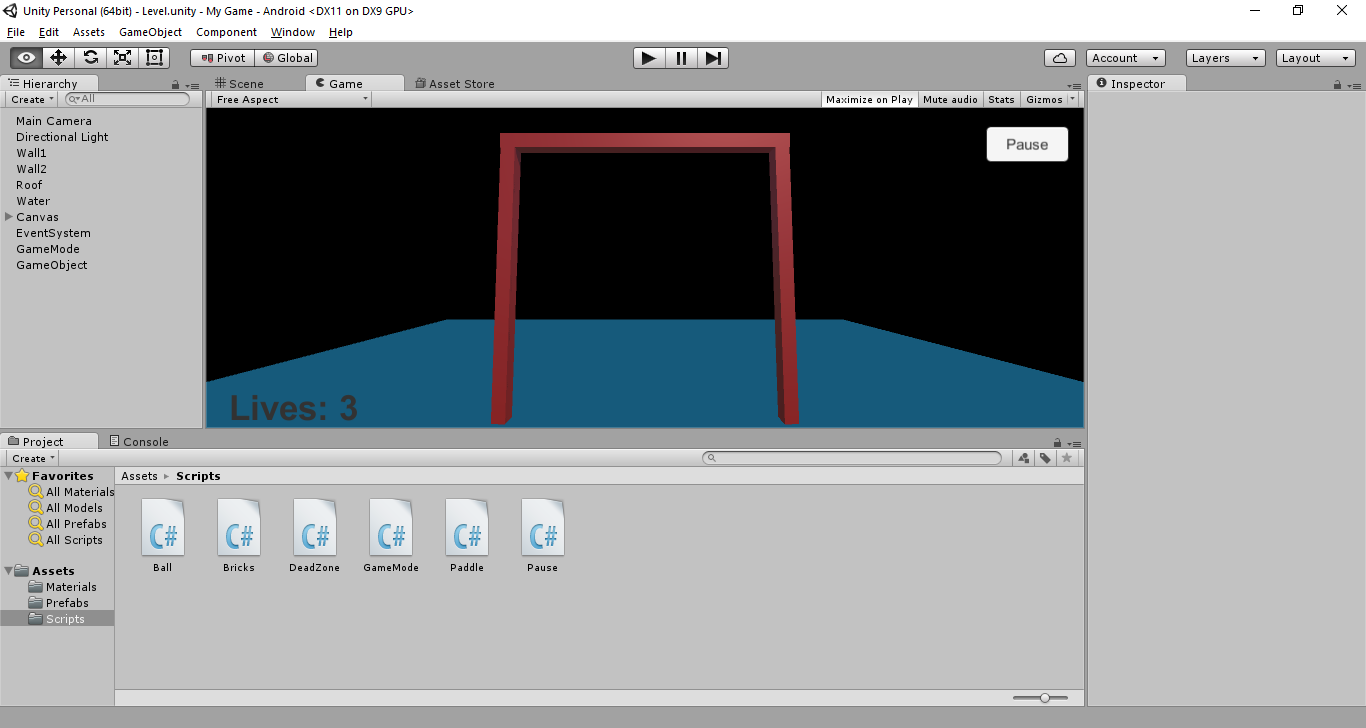
\includegraphics[scale=0.5]{images/1}
\end{center}
In imaginea de mai sus avem mai multe elmente:Game(vizualizarea scenelor finale,testarea jocurilor),Scene(aici implimentam design-ul jocului,amplasăm obiectele importate din editoare grafiece cum ar fi:Blender,3DS Max si altele,putem utiliza si obiecte primitive din Unity),Project(aici amplasam codurile,obiectele grafice in directoriile respective pentru a amenaja proectul),Inspector(este fereastra cu instructiuni pentru obiecte cum ar fi:amplasarea,rotirea etc)si Herarchy(sunt obiectele utilizate in scena curentă).\\
\begin{center}
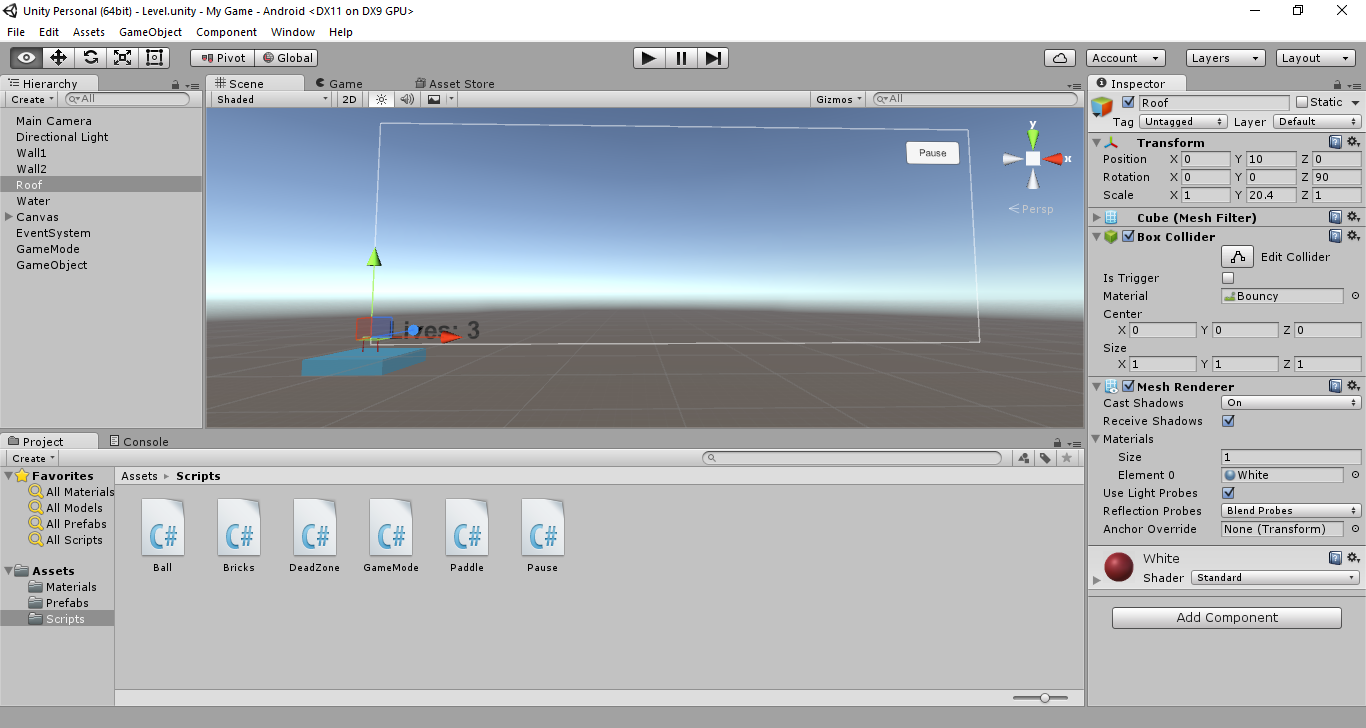
\includegraphics[scale=0.5]{images/2}\\
\end{center}
\begin{center}
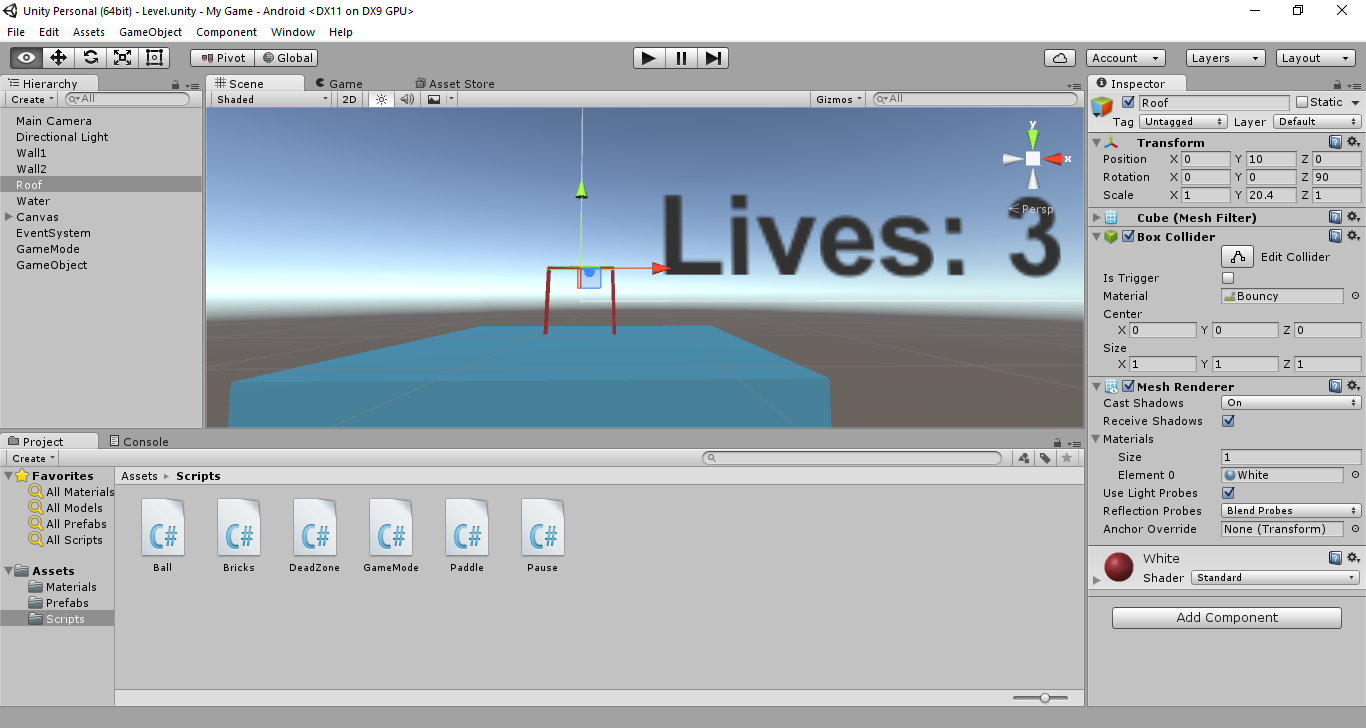
\includegraphics[scale=0.5]{images/3}\\
\end{center}
\begin{center}
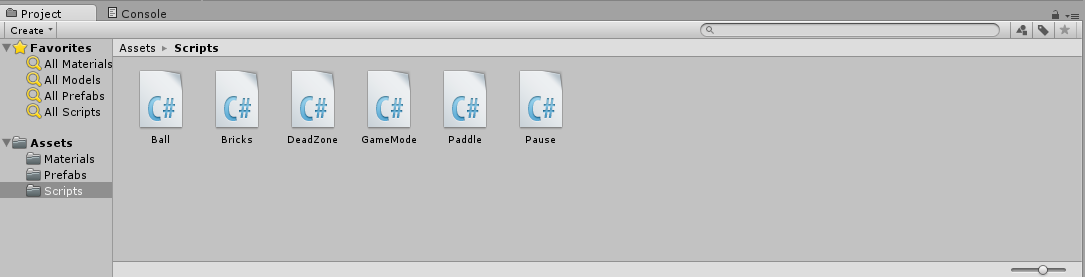
\includegraphics[scale=0.5]{images/4}\\
\end{center}

In procesul de dezvoltare a jocului putem utiliza butonul play din partea de sus pentru a testa ce am ralizat.\\
\begin{center}
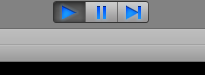
\includegraphics[scale=0.5]{images/5}\\
\end{center}

Am implementat si Meniul Pause si pagina de stop a jocului.\\
In meniul Pause sunt două butoane (unul raspunde de Repornirea jocului și al doilea pentru Iesirea din joc).\\
\begin{center}
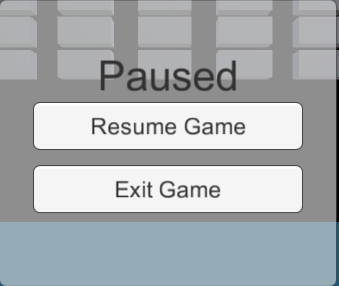
\includegraphics[scale=0.5]{images/6}\\
\end{center}
Doarece am utilizat Unity avem posibilitatea de a porta jocul pe platforma dorita doar daca avem instalate componentele necesare pentru platforma dorita ceea ce se numeste(Cross-latform).Pentru acest laborator am portat jocul doar pe platforma android.\\

\subsection{Imagini}
Imaginile finale ale jocului realizat:
\begin{center}
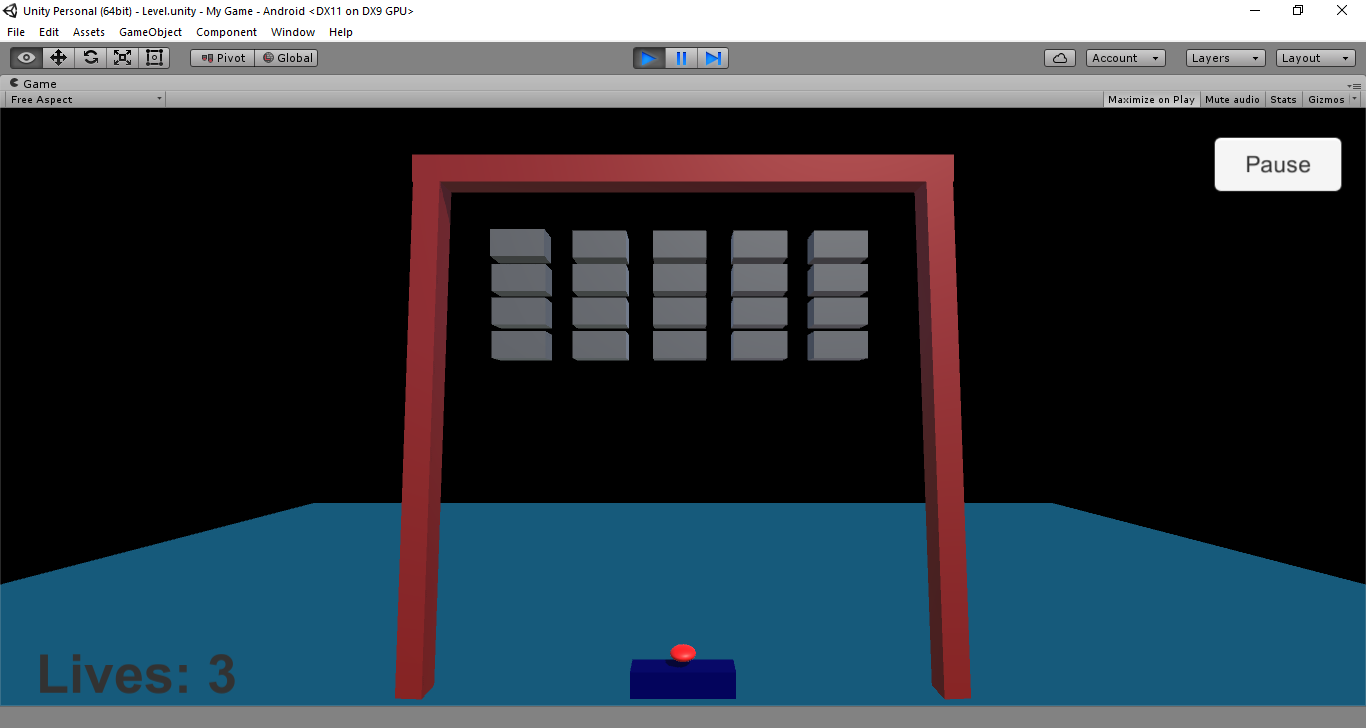
\includegraphics[scale=0.5]{images/final}\\
\end{center}
\begin{center}
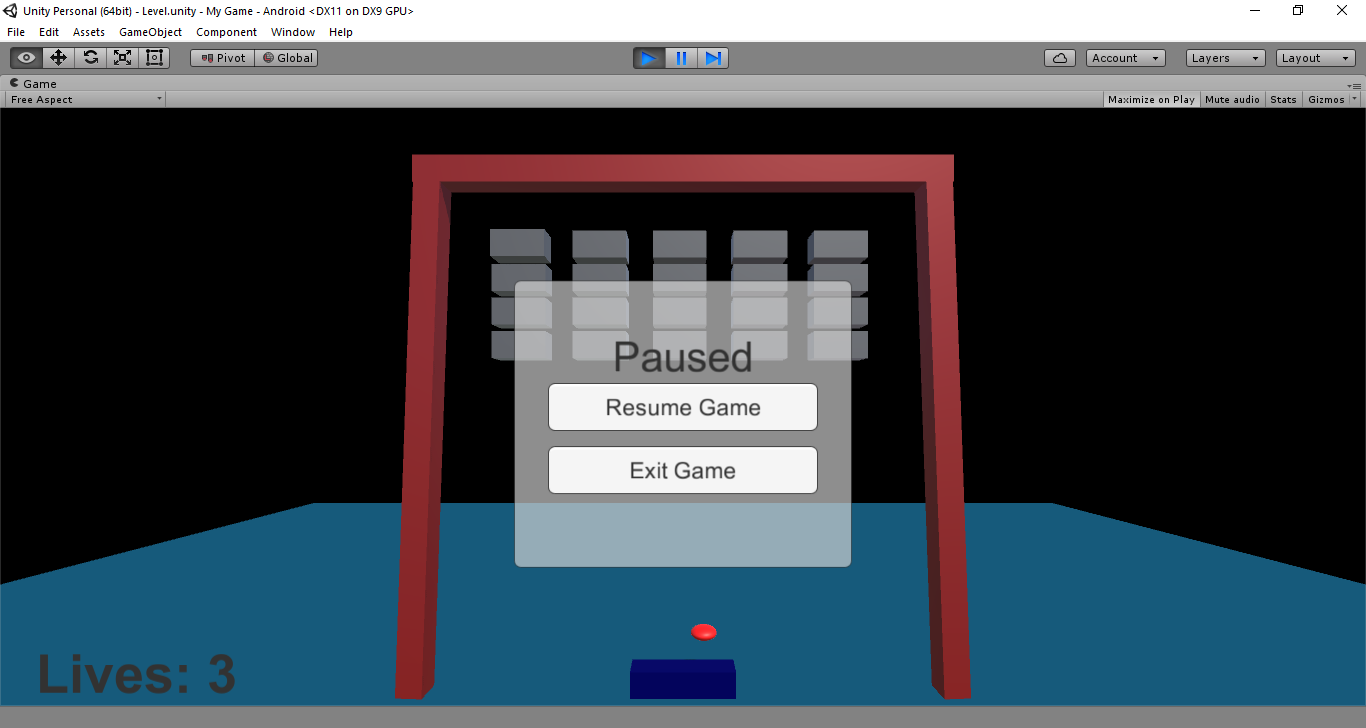
\includegraphics[scale=0.5]{images/final1}\\
\end{center}

\clearpage